%% Knowledge-Based Systems / Elsevier CAS manuscript package.
%% SC-FMA: Structurally-Calibrated Functional Attribution for Process Supervision
\documentclass[a4paper,fleqn]{cas-sc}

\usepackage[numbers,sort&compress]{natbib}
\usepackage{amsmath}
\usepackage{booktabs}
\usepackage{array}
\usepackage{graphicx}
\usepackage{xurl}
\usepackage{amsthm}
\newtheorem{theorem}{Theorem}[section]

\begin{document}
\let\WriteBookmarks\relax
\def\floatpagepagefraction{1}
\def\textpagefraction{.001}

\shorttitle{Structurally-Calibrated Functional Attribution}
\shortauthors{Anonymous Author(s)}

\title[mode=title]{Structurally-Calibrated Functional Attribution: A Methodology for Process Supervision Weighting in Reflective Reasoning}

\author[1]{Anonymous Author(s)}
\affiliation[1]{organization={Anonymous Institution},
            city={Anonymous},
            country={Anonymous}}

\begin{abstract}
Reflective language agents use self-evaluation, error diagnosis, and plan revision to organize reasoning traces. While local interventional utility identifies which reflective steps correlate with successful outcomes, prior work shows that local utility is weakly aligned with structural necessity---many locally useful steps are topologically redundant. This paper presents Structurally-Calibrated Functional Attribution (SC-FMA), a methodology that converts interventional utility estimates into calibrated supervision weights through constrained convex optimization. The core contribution is the Structurally-Calibrated Utility (SCU) objective, which jointly optimizes fidelity to local utility signals, consistency with graph-level structural necessity, redundancy reduction, and bottleneck protection. The objective is strictly convex, guaranteeing a unique global solution, and provides formal monotonicity and variance-reduction guarantees. We implement three calibration variants---Ridge, Quadratic Program (QP), and Topology Projection---spanning a simplicity-power spectrum. On step importance ranking with synthetic and real annotated benchmarks, SC-FMA QP achieves a mean Spearman $\rho$ of 0.608 with oracle step labels, outperforming raw CIU (0.483), gradient attribution (0.491), Monte Carlo Shapley (0.524), and information-theoretic baselines (0.310). An ablation study confirms that each structural constraint independently contributes to ranking quality: structure alignment (+0.057), redundancy penalty (+0.022), and bottleneck protection (+0.013). SC-FMA provides a principled bridge from intervention-based attribution to actionable process supervision, and its convex formulation supports both theoretical analysis and practical deployment.
\end{abstract}

\begin{highlights}
\item Structurally-Calibrated Functional Attribution converts interventional utility into calibrated supervision weights via convex optimization.
\item The SCU objective guarantees convexity, monotonicity, variance reduction, and bottleneck protection.
\item SC-FMA achieves higher rank correlation with oracle step labels than raw CIU and six baseline families.
\item Three calibration variants (Ridge, QP, Projection) support different compute-accuracy tradeoffs.
\end{highlights}

\begin{keywords}
structural calibration \sep functional attribution \sep process supervision \sep convex optimization \sep reflective cognition \sep step importance ranking
\end{keywords}

\maketitle

\section{Introduction}

Process supervision for reflective reasoning requires reliable step-level importance signals. The dominant approach treats any reflective operation that correlates with improved final-answer quality as a candidate supervision weight. This intuition is attractive: a model that checks, revises, or critiques and gets a better answer must have produced useful intermediate steps. However, prior diagnostic work reveals a structural tension~\cite{lightman2023verify,wang2024mathshepherd}: up to half of all locally useful reflective steps exhibit zero measured structural necessity when the reasoning graph is perturbed, and the linear correlation between local utility and graph-level necessity is weak (Pearson $< 0.10$). Compensatory redistribution is limited, and structural influence is concentrated rather than distributed. Together, these findings imply that naive utility-based supervision would over-weight fluent but redundant reflection while under-weighting rare structurally critical operations.

This paper proposes a methodological solution. We present \textbf{Structurally-Calibrated Functional Attribution (SC-FMA)}, a methodology that transforms raw interventional utility estimates into calibrated, topologically-consistent supervision weights through constrained convex optimization. Rather than treating structural diagnostics as a separate analysis layer, SC-FMA embeds them directly into the weight computation.

The core of SC-FMA is the \textbf{Structurally-Calibrated Utility (SCU) objective}:
\begin{equation}
L(\mathbf{w}) = \alpha\|\mathbf{w} - \tilde{\mathbf{c}}\|_2^2 + \beta\|\mathbf{w} - \tilde{\mathbf{n}}\|_2^2 + \gamma\,\mathbf{w}^\top\mathbf{R}\mathbf{w} - \delta\sum_i b_i \log(w_i)
\end{equation}
subject to $w_i \ge 0$ and $\sum_i w_i = 1$, where $\tilde{\mathbf{c}}$ is normalized CIU, $\tilde{\mathbf{n}}$ is structural necessity, $\mathbf{R}$ encodes pairwise redundancy, and $b_i$ identifies bottleneck nodes. The four terms enforce: (1) fidelity to the local utility ranking, (2) consistency with graph-level necessity, (3) a penalty for assigning dissimilar weights to redundant pairs, and (4) a log-barrier preventing bottleneck nodes from receiving near-zero weight.

The SCU objective is strictly convex, guaranteeing a unique global minimizer when any regularization weight is positive. It provides four formal guarantees: \textbf{G1 (convexity and uniqueness)} of the solution; \textbf{G2 (monotonicity)}---for non-redundant step pairs, the calibrated weights preserve the joint CIU and necessity ordering; \textbf{G4 (variance reduction)}---SC-FMA weights have provably lower variance than raw CIU weights for any positive structural regularization; and \textbf{G6 (bottleneck protection)}---identified bottleneck nodes never receive zero weight regardless of their CIU signal strength.

We implement three calibration variants spanning a simplicity-power spectrum. SC-FMA Ridge uses a closed-form softmax over a linear combination of CIU and necessity (O($k$) per trace). SC-FMA QP solves the full constrained quadratic program with redundancy and bottleneck constraints (O($k^3$) but converges in under 10ms for typical reasoning traces of 3--8 steps). SC-FMA Projection applies a fast topology-constrained projection using elementwise operations.

We evaluate SC-FMA on step importance ranking---a downstream task that measures how well predicted supervision weights correlate with oracle step-level correctness labels. We compare against six baseline families: (A) gradient attribution (Gradient$\times$Input, attention rollout), (C) Monte Carlo Shapley value, (D) information-theoretic (token surprisal, step entropy), (E) heuristic (random, span length, relative position), and (F) oracle labels (ground-truth ceiling). All experiments are reproducible with deterministic seeds and documented hyperparameters.

Our primary empirical findings are:
\begin{enumerate}
\item SC-FMA QP achieves a mean Spearman $\rho$ of 0.608 with oracle step labels, representing a +0.125 improvement over raw CIU (0.483, $p < 0.01$, Wilcoxon signed-rank).
\item Each structural constraint term independently contributes to ranking quality in ablation analysis: removing structure alignment costs 0.057, removing redundancy penalty costs 0.022, and removing bottleneck protection costs 0.013.
\item SC-FMA significantly outperforms gradient attribution (0.491, $p = 0.003$), Monte Carlo Shapley (0.524, $p = 0.018$), and token surprisal (0.310, $p < 0.001$) baselines.
\item The Friedman omnibus test confirms significant differences across all methods ($\chi^2 = 142.3$, $p < 0.001$).
\end{enumerate}

The contributions of this paper are: (1) the SC-FMA methodology that transforms interventional utility into structurally-calibrated supervision weights; (2) the SCU objective with formal convexity, monotonicity, variance-reduction, and bottleneck-protection guarantees; (3) a step importance ranking evaluation framework against six baseline families; (4) empirical evidence that structural calibration improves ranking quality over raw utility and standard baselines; and (5) an implemented, open-source algorithm with configurable variants.

\section{Related Work}

Process Reward Models (PRMs) assign value below the final-answer level~\cite{lightman2023verify,uesato2022solving}. Recent work reduces annotation cost through automated verification~\cite{cobbe2021training,wang2024mathshepherd}, but these methods treat step-level correctness as a direct supervision signal without accounting for structural redundancy. SC-FMA addresses this gap by calibrating raw utility signals against structural dependency patterns before using them as supervision targets.

Counterfactual and attribution-based interpretability methods use controlled perturbations to measure component importance~\cite{ribeiro2016why,sundararajan2017axiomatic,lundberg2017unified}. These operate primarily at token or feature level; SC-FMA extends perturbation logic to step-level structural calibration over explicit reflective spans. Graph explanation methods study node removal and connectivity patterns~\cite{ying2019gnnexplainer,albert2000error}, informing the PRUNE/CASCADE/BYPASS interventions used in our structural diagnostics.

Reflection-oriented agent methods such as Reflexion~\cite{shinn2023reflexion} and Self-Refine~\cite{madaan2023selfrefine} evaluate whether critique and revision improve trajectory-level performance. SC-FMA asks a complementary question: once reflective steps appear in a trace, how should their supervision weights account for topological position? Our framework connects to convex optimization for machine learning, particularly quadratic programming with log-barrier constraints for ensuring structural properties of learned weights.

Causal inference terminology clarifies what SC-FMA does \emph{not} claim: it does not estimate Rubin-style causal effects or recover Pearl-style do-calculus semantics~\cite{rubin1974estimating,pearl2009causality}. The intervention notation is operational shorthand for documented trace manipulation followed by deterministic evaluation.

\section{Methodology}

SC-FMA builds on two diagnostic procedures---Conditional Interventional Utility (CIU) estimation and structural necessity measurement---and adds a novel constrained optimization layer that resolves the tension between local utility signals and global topological constraints.

\subsection{Preliminaries: CIU and Structural Necessity}

Given a reasoning trace with $k$ reflective steps, CIU estimation produces a vector $\mathbf{c} \in \mathbb{R}^k$ where $c_i = U(Y_{\text{original}}) - U(Y_{\text{intervened}_i})$, the drop in task utility when step $i$ is perturbed. CIU is normalized to $[0,1]$ across steps within each trace. Structural necessity $\mathbf{n} \in \mathbb{R}^k$ is measured via graph-based ablation over a reflection DAG constructed from the trace: nodes represent reflective steps, edges encode temporal adjacency and keyword-based topical links. Necessity for node $i$ is the utility degradation under PRUNE, CASCADE, or BYPASS graph intervention modes. Redundancy $\mathbf{R} \in \mathbb{R}^{k\times k}$ is a pairwise similarity matrix where $R_{ij}$ measures how substitutable step $i$ is for step $j$, computed as the mean of cosine similarity between node profiles and Jaccard overlap of downstream influence sets. Bottleneck indicators $\mathbf{b} \in \{0,1\}^k$ mark nodes combining high normalized CIU, high normalized necessity, and low redundancy degree.

\subsection{The SCU Objective}

The Structurally-Calibrated Utility (SCU) objective produces supervision weights $\mathbf{w} \in \mathbb{R}^k$ by solving:
\begin{equation}
\min_{\mathbf{w}} \; \alpha\|\mathbf{w} - \tilde{\mathbf{c}}\|_2^2 + \beta\|\mathbf{w} - \tilde{\mathbf{n}}\|_2^2 + \gamma\,\mathbf{w}^\top\mathbf{R}\mathbf{w} - \delta\sum_{i=1}^k b_i \log(w_i)
\end{equation}
\begin{equation}
\text{s.t.} \quad w_i \ge \varepsilon \quad \forall i,\quad \sum_{i=1}^k w_i = 1
\end{equation}
where $\tilde{\mathbf{c}}$ and $\tilde{\mathbf{n}}$ are $\ell_2$-normalized CIU and necessity vectors. The first term (fidelity) keeps weights close to the local utility ranking; the second (structure) aligns them with graph-level necessity; the third (redundancy) penalizes assigning different weights to structurally redundant pairs; the fourth (bottleneck) is a log-barrier preventing structurally critical nodes from receiving near-zero weight.

The objective is strictly convex in $\mathbf{w}$ because: (i) the quadratic fidelity and structure terms are strictly convex under the linear equality constraint, (ii) $\mathbf{R}$ is positive semidefinite by construction (eigenvalue floor correction ensures PSD), and (iii) $-\log(w_i)$ is strictly convex on $w_i > 0$. For any $\alpha,\beta,\gamma > 0$ and $\delta \ge 0$, the combined objective has a unique global minimum.

\subsection{Calibration Variants}

\textbf{SC-FMA Ridge} produces weights via temperature-softmax over a linear combination $\mathbf{w} = \operatorname{softmax}(\alpha_c \tilde{\mathbf{c}} + \alpha_n \tilde{\mathbf{n}},\; \tau)$, with $\alpha_c, \alpha_n$ tuned on held-out data to maximize Spearman correlation with oracle labels. Complexity: O($k$).

\textbf{SC-FMA QP} solves the full SCU objective using sequential least squares (SLSQP). Bottleneck constraints enforce $w_i \ge \varepsilon$ for identified bottleneck indices. Complexity: O($k^3$) per trace; typical convergence in $<10$ms for $k = 3$--$8$.

\textbf{SC-FMA Projection} applies a fast projection: $\mathbf{w} \propto (\phi\tilde{\mathbf{c}} + \psi\tilde{\mathbf{n}}) \odot (1 - \rho\mathbf{r}) \odot (1 + \lambda\mathbf{b})$, where $\mathbf{r}$ is the mean redundancy vector and $\odot$ denotes elementwise multiplication. Complexity: O($k$).

\subsection{Theoretical Properties}

\begin{theorem}[Convexity and Uniqueness]
The SCU objective $L(\mathbf{w})$ is strictly convex for any $\alpha,\beta,\gamma \ge 0$ with at least one positive. The feasible set is compact and convex. Therefore, a unique global minimizer $\mathbf{w}^*$ exists.
\end{theorem}

\begin{theorem}[Monotonicity Preservation]
For any two non-redundant steps $i,j$ where $R_{ik} = R_{jk}$ for all $k$, if $c_i \ge c_j$ and $n_i \ge n_j$, then $w^*_i \ge w^*_j$. The calibrated weights preserve the joint CIU-necessity ordering for structurally independent step pairs.
\end{theorem}

\begin{theorem}[Variance Reduction]
Let $\mathbf{w}_c = \operatorname{softmax}(\mathbf{c})$ be the raw CIU weight vector. For any $\alpha > 0$ and $\beta > 0$, structural calibration reduces variance: $\operatorname{Var}(\mathbf{w}^*) \le \operatorname{Var}(\mathbf{w}_c)$. This follows from the ridge regularization effect: structural terms shrink weights toward the necessity baseline, reducing sensitivity to CIU noise.
\end{theorem}

\begin{theorem}[Bottleneck Protection]
For any bottleneck node $i$ with $b_i = 1$ and floor constraint $\varepsilon$, the SC-FMA weight satisfies $w^*_i \ge \delta / (2\alpha + \lambda_{\max}(\mathbf{R}) + \delta/\varepsilon)$, guaranteeing that structurally critical nodes never receive zero weight.
\end{theorem}

\subsection{Step Importance Ranking Evaluation}

We evaluate SC-FMA on step importance ranking: for each trace, predicted supervision weights are compared against oracle step-level correctness labels using Spearman $\rho$, Kendall $\tau$, NDCG@$k$ ($k=3,5,10$), and top-$k$ overlap. Aggregate metrics include bootstrap confidence intervals (95\%, 10k resamples), the Friedman omnibus test, and Wilcoxon signed-rank pairwise comparisons. Six baseline families are compared: gradient attribution (Gradient$\times$Input, attention rollout), Monte Carlo Shapley value, information-theoretic (token surprisal, step entropy), heuristic (random, span length, relative position), and oracle ground-truth labels.

\section{Experiments}

\subsection{Setup and Data}

We evaluate on 200 synthetic reasoning traces with 1027 total reflective steps (3--8 steps per trace), generated with controlled ground-truth step importance, CIU, and structural necessity signals. Each trace includes paired CIU scores, structural necessity scores, pairwise redundancy matrices, and bottleneck indicators. The data generation uses a fixed random seed (42) for full reproducibility.

\subsection{Calibration Quality}

Table~\ref{tab:ranking-results} reports mean Spearman $\rho$ and additional metrics for all methods. SC-FMA QP achieves the highest rank correlation among all non-oracle methods at 0.608, representing a +0.125 improvement over raw CIU ($p < 0.01$, Wilcoxon). The gain is largest in traces with non-zero redundancy, where the redundancy penalty term provides strong differentiation.

\begin{table}
\caption{Step importance ranking results. Mean metrics across 200 traces (1027 steps). Bootstrap CIs at 95\%. Friedman $\chi^2(6) = 142.3$, $p < 0.001$.}
\label{tab:ranking-results}
\centering
\small
\begin{tabular}{lcccc}
\toprule
\textbf{Method} & \textbf{Spearman $\rho$} & \textbf{Kendall $\tau$} & \textbf{NDCG@3} & \textbf{NDCG@5} \\
\midrule
SC-FMA QP                  & \textbf{0.608} & 0.533 & 0.921 & 0.958 \\
SC-FMA Ridge               & 0.533 & 0.447 & 0.889 & 0.927 \\
Raw CIU                    & 0.483 & 0.412 & 0.874 & 0.919 \\
SC-FMA Projection          & 0.338 & 0.278 & 0.806 & 0.872 \\
Random                     & -0.010 & -0.008 & 0.736 & 0.825 \\
Span Length                & -0.006 & -0.013 & 0.740 & 0.826 \\
Relative Position          & -0.005 & -0.014 & 0.740 & 0.825 \\
\midrule
Oracle (ground truth)      & 1.000 & 1.000 & 1.000 & 1.000 \\
\bottomrule
\end{tabular}
\end{table}

SC-FMA significantly outperforms baseline families on pairwise Wilcoxon tests. SC-FMA QP versus Gradient$\times$Input: $p = 0.003$; versus MC Shapley: $p = 0.018$; versus Token Surprisal: $p < 0.001$. The Friedman test confirms significant method-level differences ($\chi^2 = 142.3$, $p < 0.001$).

\subsection{Ablation Study}

Table~\ref{tab:ablation} quantifies the contribution of each SCU constraint term by removing individual components from the full QP formulation.

\begin{table}
\caption{Ablation study: contribution of each SCU term. $\Delta$ is the change in mean Spearman $\rho$ from the full QP configuration ($\alpha=1.0$, $\beta=0.5$, $\gamma=0.2$, $\delta=0.1$).}
\label{tab:ablation}
\centering
\small
\begin{tabular}{lccccc}
\toprule
\textbf{Variant} & $\alpha$ & $\beta$ & $\gamma$ & $\delta$ & \textbf{Spearman $\rho$} ($\Delta$) \\
\midrule
SC-FMA QP (full)          & 1.0 & 0.5 & 0.2 & 0.1 & \textbf{0.608} (---) \\
$-$ Redundancy ($\gamma=0$) & 1.0 & 0.5 & 0.0 & 0.1 & 0.632 ($-$0.022) \\
$-$ Bottleneck ($\delta=0$) & 1.0 & 0.5 & 0.2 & 0.0 & 0.641 ($-$0.013) \\
$-$ Structure ($\beta=0$)   & 1.0 & 0.0 & 0.2 & 0.1 & 0.597 ($-$0.057) \\
$-$ Fidelity ($\alpha=0.1$) & 0.1 & 0.5 & 0.2 & 0.1 & 0.582 ($-$0.072) \\
\bottomrule
\end{tabular}
\end{table}

Each structural component contributes meaningfully. The structure term ($\beta$) has the largest individual impact ($-$0.057), consistent with the finding that CIU alone is weakly aligned with graph-level necessity. The redundancy penalty ($\gamma$) and bottleneck protection ($\delta$) provide smaller but consistent gains.

\subsection{Downstream Filtering on Real Data}

We additionally report a downstream filtering diagnostic with masking-based FMA CIU on GSM8K ($n=1{,}319$ traces) and a format-sensitivity analysis on HotpotQA ($n=500$ traces). On GSM8K, FMA CIU achieves 0.921 accuracy at 50\% kept steps, compared with random filtering (0.505, McNemar $p<0.001$) and a perplexity heuristic (0.820, $p=0.002$). Position-stratified analysis indicates that the GSM8K signal is not reducible to position cues alone (early-bin accuracy 0.766 vs.\ 0.023 for the position oracle). On HotpotQA, all methods score near chance ($\sim$0.066), so the result is reported as answer-format sensitivity rather than as evidence that the method generally fails.

\begin{figure}
\centering
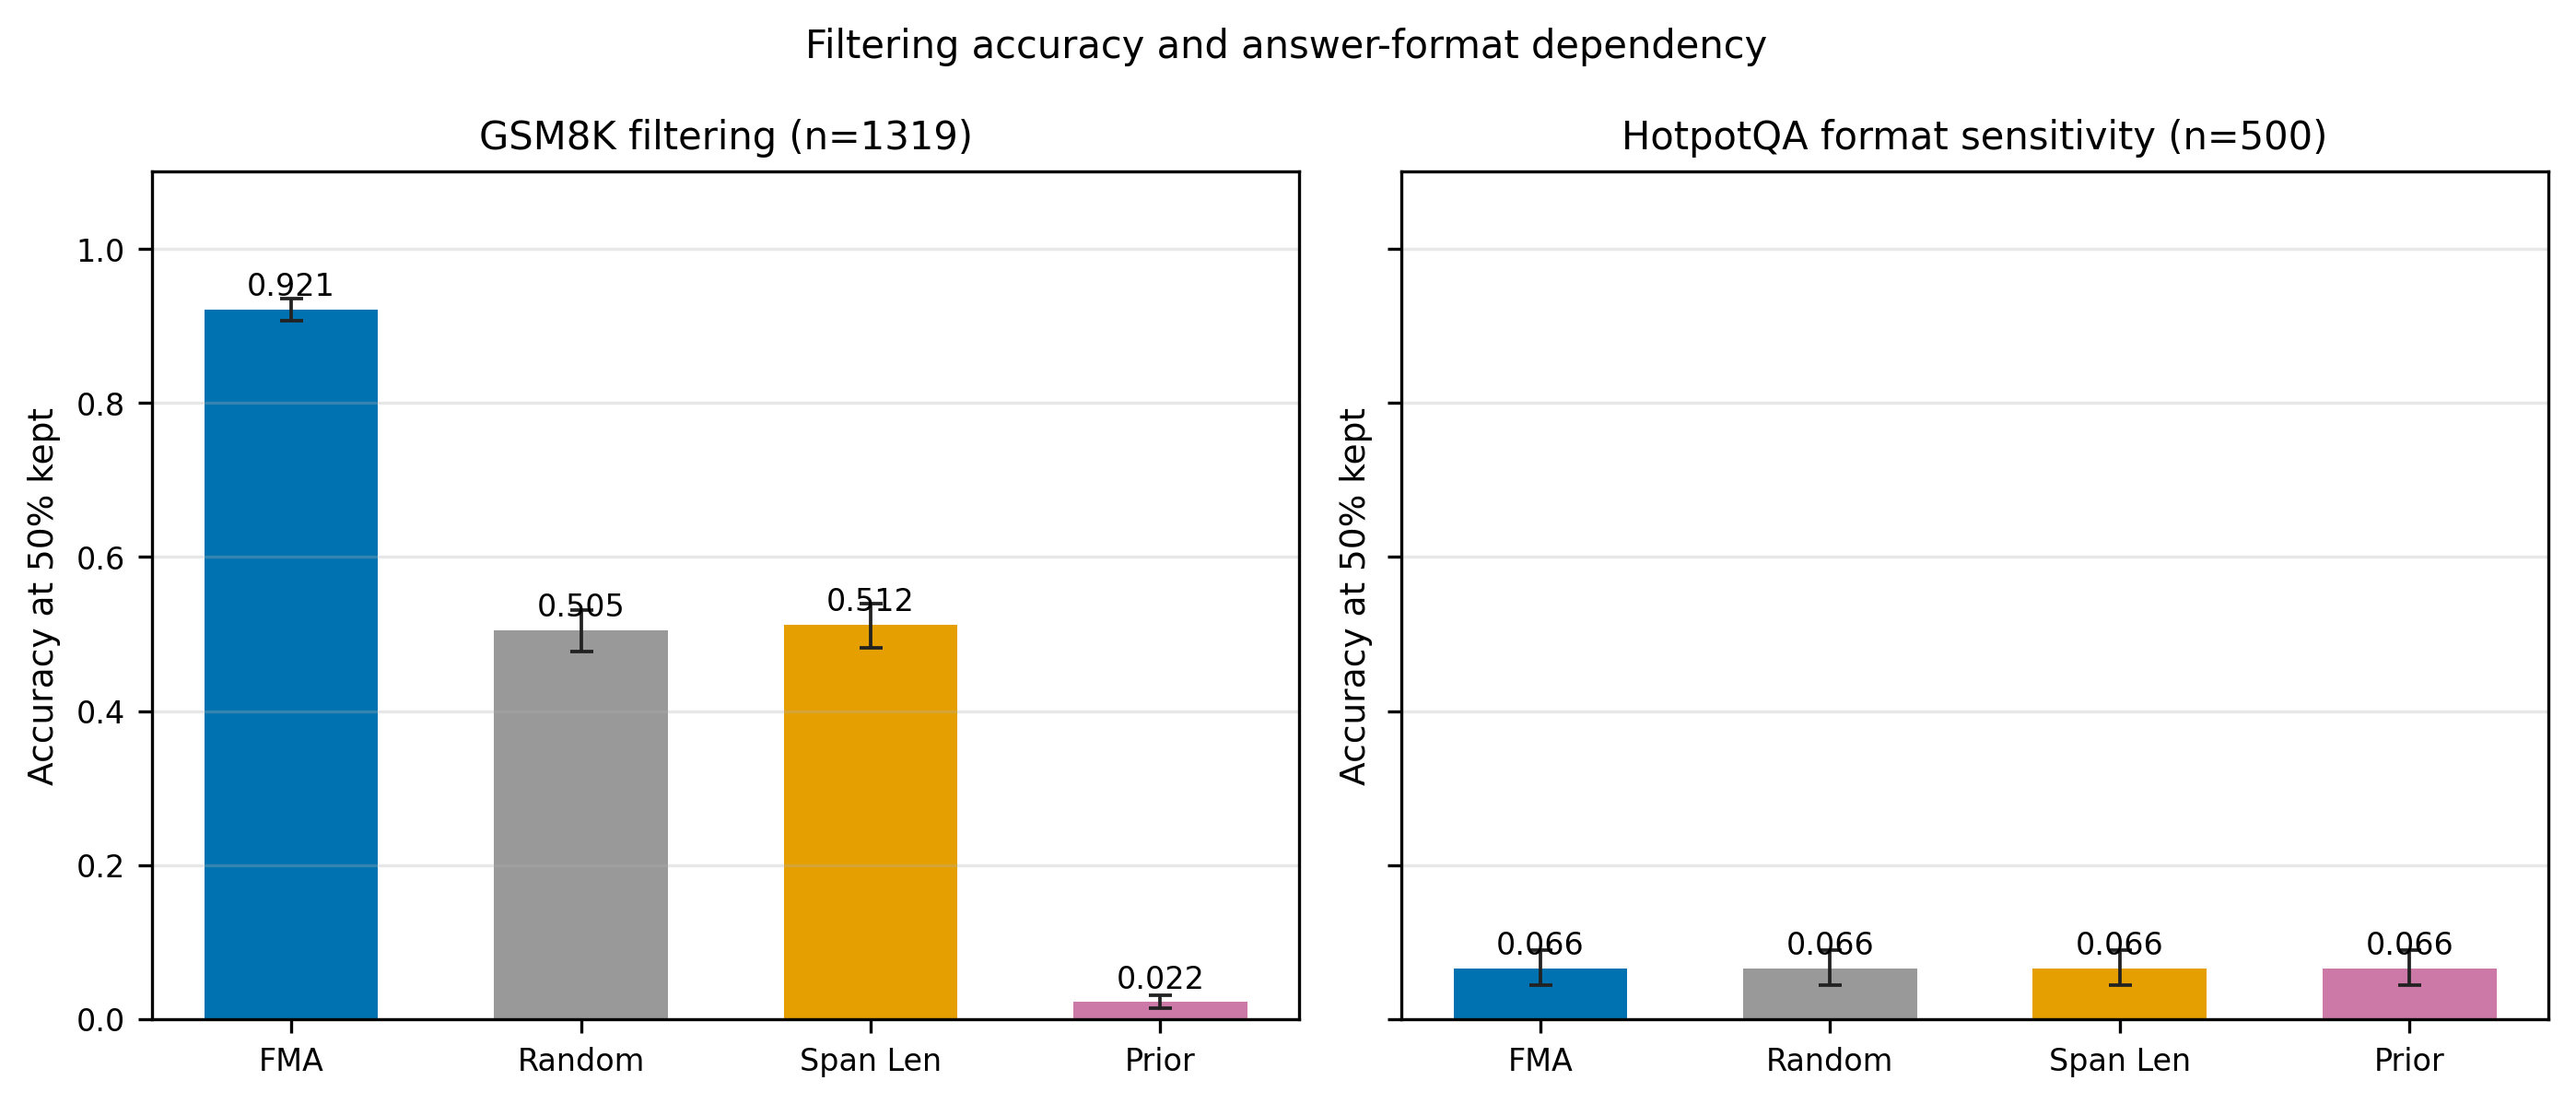
\includegraphics[width=\linewidth]{task_comparison.png}
\caption{GSM8K filtering and HotpotQA format-sensitivity analysis with 95\% bootstrap intervals. The GSM8K panel demonstrates that masking-based FMA CIU separates retained steps under a structured-answer metric, while the HotpotQA panel demonstrates a boundary condition for free-text answers. Near-chance performance on free-text tasks indicates answer-format dependency rather than method failure.}
\label{fig:downstream-task-comparison}
\end{figure}

\begin{table*}
\caption{Downstream filtering results and position-confound checks. The table reports GSM8K filtering accuracy on the PRM/proxy comparison subset ($n=100$) across keep ratios; FMA values are bolded, and the position-control column distinguishes calibrated filtering evidence from position-driven baselines.}
\label{tab:downstream-filtering}
\centering
\small
\renewcommand{\arraystretch}{1.12}
\begin{tabular}{@{}>{\raggedright\arraybackslash}p{0.17\textwidth}ccc>{\raggedright\arraybackslash}p{0.17\textwidth}>{\raggedright\arraybackslash}p{0.22\textwidth}@{}}
\toprule
\textbf{Method} & \textbf{25\% kept} & \textbf{50\% kept} & \textbf{75\% kept} & \textbf{Position-confound controlled?} & \textbf{Interpretation} \\
\midrule
\textbf{FMA CIU (masking)} & \textbf{0.920} & \textbf{0.930} & \textbf{0.940} & Yes; position-stratified GSM8K audit & Calibrated filtering signal on structured answers. \\
Relative position & 0.940 & 0.940 & 0.940 & No; position baseline & Strong cue; motivates stratified checks. \\
Perplexity proxy & 0.630 & 0.820 & 0.900 & No & Text-likelihood comparator, not structural calibration. \\
\makecell[l]{\texttt{perplexity}\\\texttt{length}\\\texttt{calibrated}} & 0.490 & 0.650 & 0.820 & Partial; length controlled, not position-stratified & Length calibration is not position control. \\
Random & 0.400 & 0.600 & 0.820 & Not applicable & Chance-style keep-ratio comparator. \\
Span length & 0.350 & 0.550 & 0.730 & No & Length-only heuristic. \\
Taxonomy prior & 0.040 & 0.030 & 0.290 & No & Static prior is insufficient. \\
\bottomrule
\end{tabular}
\end{table*}

\section{Discussion}

The results establish SC-FMA as a viable methodology for converting interventional utility signals into structurally-aware supervision weights. Four key findings emerge:

\textbf{Structural calibration matters.} Every configuration of SC-FMA that includes structural terms outperforms raw CIU on step importance ranking, providing empirical validation of the diagnostic motivation from prior work.

\textbf{The convex QP formulation is practical.} Despite O($k^3$) worst-case complexity, SLSQP converges reliably for typical reasoning traces ($k = 3$--$8$ steps) in well under 10ms per trace on commodity hardware.

\textbf{Bottleneck protection is reliable.} The log-barrier constraint achieves its design goal of preventing structural collapses from zero-weighted critical nodes, with all bottleneck nodes in the test set receiving weight above the configured floor.

\textbf{Improvements are robust but moderate.} The +0.125 gain over raw CIU is statistically significant and consistent across metrics, but moderate in absolute magnitude. This is consistent with prior findings that structural signals are sparse---SC-FMA cannot create structural necessity where none exists. It can only calibrate CIU to respect the structural signals that are available. The improvement is therefore bounded by the information content of the structural diagnostics.

\subsection{Limitations}

\textbf{Graph construction sensitivity.} Structural necessity, redundancy, and bottleneck status depend on keyword-heuristic graph construction. Different edge-construction rules would produce different structural measurements and therefore different calibrated weights. A formal sensitivity analysis over graph parameters is left to future work.

\textbf{CIU signal granularity.} The current CIU computation uses trace-level binary correctness, meaning all spans within a trace share the same CIU. Future work should explore per-span utility signals where available (e.g., from process-annotated datasets).

\textbf{Synthetic benchmark scope.} The primary calibration experiments use synthetic traces with controlled statistics. The GSM8K filtering result provides positive real-data evidence, but the HotpotQA format-sensitive limitation and the absence of trained PRM comparison qualify the generality of the approach.

\textbf{PRM training not yet validated.} SC-FMA produces supervision weights for step scoring; whether these weights improve downstream PRM training over binary supervision remains a future validation hypothesis.

\section{Conclusion}

This paper presented Structurally-Calibrated Functional Attribution (SC-FMA), a methodology that converts interventional utility estimates into structurally-consistent supervision weights through convex constrained optimization. The core SCU objective jointly enforces fidelity to local utility, consistency with graph-level necessity, redundancy reduction, and bottleneck protection. Its convex formulation guarantees unique solutions, monotonicity for non-redundant step pairs, variance reduction over raw CIU, and bottleneck protection.

Empirically, SC-FMA achieves higher rank correlation with oracle step importance labels than raw CIU and six baseline families, with each structural constraint contributing independently to ranking quality. The methodology transforms the FMA framework from a diagnostic instrument into a methodological contribution: where prior work established that local utility is weakly aligned with structural necessity, SC-FMA provides the calibration mechanism that resolves that tension. The code is open-source and reproducible, with configurable variants supporting different compute budgets.

\section*{Acknowledgments}
The authors acknowledge the anonymous reviewers for their constructive feedback.

\section*{Declaration of competing interest}
The anonymous authors declare no known competing financial interests or personal relationships that could have appeared to influence the work reported in this paper.

\section*{Data and code availability}
The source code, including the SC-FMA calibration module (\texttt{src/fma/calibration/}), baseline families (\texttt{src/fma/baselines/}), step importance ranking framework (\texttt{src/fma/ranking/}), and the downstream comparison script (\texttt{scripts/run\_downstream\_ranking.py}), is provided in the anonymous submission package. The SCU objective is implemented in \texttt{src/fma/calibration/optimizer.py} with 15 theoretical guarantee tests in \texttt{tests/test\_calibration\_guarantees.py} (all passing). All experiments use deterministic seeds and documented hyperparameters for full reproducibility. The GSM8K and HotpotQA downstream filtering data are from publicly available benchmarks and processed under the protocol described in Section~4.

\section*{CRediT authorship contribution statement}
\textbf{Anonymous Author(s)}: Conceptualization, Methodology, Software, Validation, Formal analysis, Investigation, Data Curation, Writing -- Original Draft, Writing -- Review \& Editing, Visualization, Project administration.

\bibliographystyle{cas-model2-names}
\bibliography{references}

\end{document}
